\setcounter{section}{39}
\section{Дерево поиска: определения и операции find, insert, erase, merge, split}

\textbf{Опр} Бинарное дерево поиска (англ. binary search tree, BST) - структура данных для работы с упорядоченными множествами.
Бинарное дерево поиска обладает следующим свойством: если x - узел бинарного дерева с ключом k, то все узлы в левом поддереве должны иметь ключи, меньшие k, а в правом поддереве большие k.

\begin{figure}[h]
\center{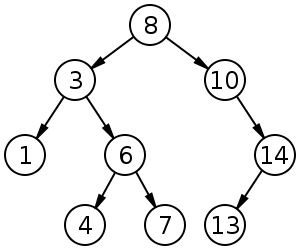
\includegraphics[width=5cm]{images/40-42_binary_search_tree.svg.png}}
\caption {Binary tree}
\label{ris:image}
\end{figure}

\subsection*{Операции }
\textbf{Find: }

Для поиска элемента в бинарном дереве поиска можно воспользоваться функцией \textit{find(node* root, int key)}, которая принимает в качестве параметров корень дерева и искомый ключ. Для каждого узла функция сравнивает значение его ключа с искомым ключом. Если ключи одинаковы, то функция возвращает текущий узел, в противном случае функция вызывается рекурсивно для левого или правого поддерева(если искомое значение больше, то от правого, иначе - от левого). Узлы, которые посещает функция образуют нисходящий путь от корня, так что время ее работы O(h), где h — высота дерева.

\begin{lstlisting}
   Node find (Node x, int key){
        if (x == nullptr || x.key = key) return x;

        if (key < x.key) return find(x.left, key);
        else return find(x.right, key);
            
        }
\end{lstlisting}

\textbf{Insert: }

Операция вставки работает аналогично поиску элемента, только спуск происходит до тех пор, пока у текущей вершины не будет  отсутствовать лист, в который мы хотим спустится. Тогда на месте пустой вершины мы и подвешиваем узел.

\textbf{Erase: }

Рассмотрим 3 возможных случая расположения вершины, которую мы хотим удалить, в дереве:
\begin{itemize}
    \item[1] Если у узла нет дочерних узлов, то у его родителя нужно просто заменить указатель на nullptr
    \item[2]  Если у узла есть только один дочерний узел, то нужно создать новую связь между родителем удаляемого узла и его дочерним узлом.
    \item[3] Если у узла два дочерних узла, то нужно найти следующий за ним элемент (т.е. минимальный элемент в поддереве). У минимального элемента в поддерве нет левого потомка. Правого потомка подвешиваем на место минимального элемента. А удаляемый элемент заменяем минимальным. 
      \end{itemize}
   
\begin{figure}[h]
\center{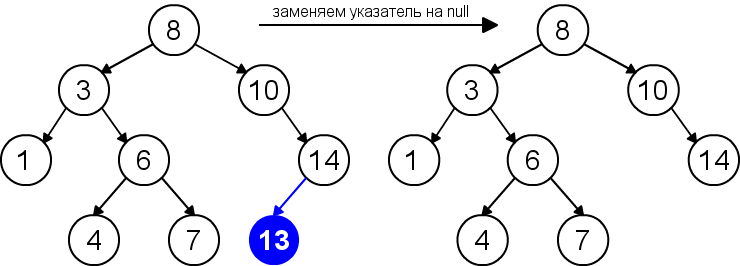
\includegraphics[width=7cm]{images/40-42_bst_del1.png}}
\caption {1 случай}
\end{figure}
\begin{figure}[h]
\center{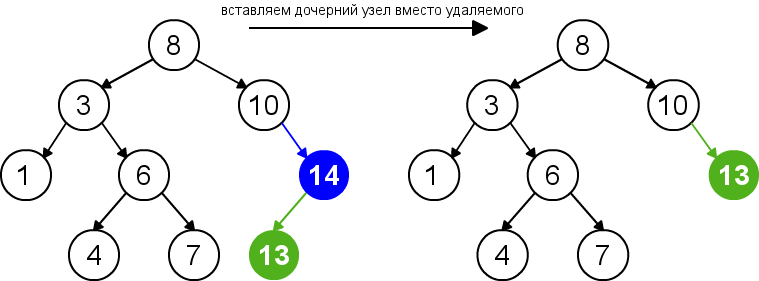
\includegraphics[width=7cm]{images/40-42_bst_del2.png}}
\caption {2 случай}
\end{figure}
\begin{figure}[h]
\center{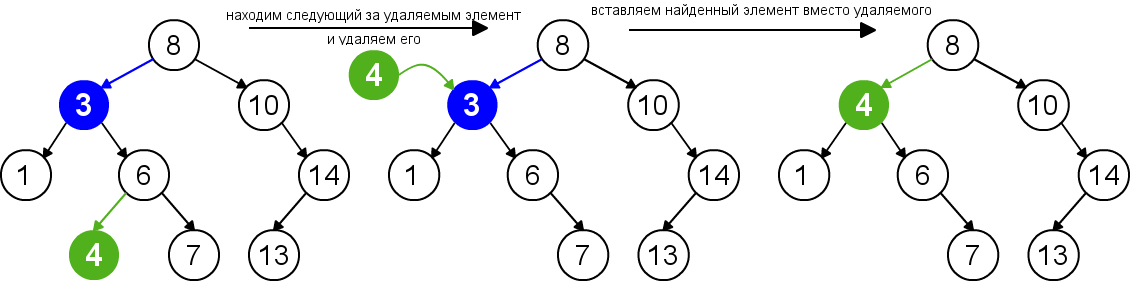
\includegraphics[width=7cm]{images/40-42_bst_del3.png}}
\caption {3 случай}
\label{ris:image}
\end{figure}

\textbf{Merge: }

Merge (слияние) - операция, которая может быть реализована для декартовых деревьев, все значения одного из которых не превосходят значений второго или для любых splay деревьев. 
Примитивно можно по одному добавлять элементы из одного дерева в другое.

\textbf{Split: }

Операция разбиения дерева на два по ключу так, чтобы в одном дереве все элементы были <= key, а в другом > key (неравенства могут быть и другие) . Также может быть реализована для декартовых и splay деревьев. 

\setcounter{section}{40}
\section{Большие и малые повороты в дереве поиска}

\textbf{Опр} Повороты - это специальные балансирующие операции, восстанавливающие основное свойство дерева: «высоты двух поддеревьев различаются не более чем на 1».

\begin{itemize}
    \item Малый левый поворот
    \item Малый правый поворот
    \item Большой левый поворот
    \item Большой правый поворот
\end{itemize}

\subsubsection*{Малый левый поворот}

\begin{itemize}
    \item Используется, когда $H(R) = H(L) + 2$ и $H(C)$ не больше $H(R)$
    \item После операции:
    \\
    высота дерева останется прежней, если $H(C) = H(R)$,
    \\
    высота дерева уменьшится на 1, если $H(C) < H(R)$.
\end{itemize}

\begin{figure}[h]
\center{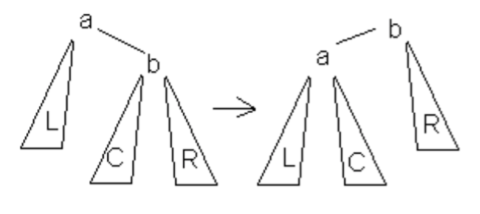
\includegraphics[width=7cm]{images/40-42_5.png}}
\end{figure}

\subsubsection*{Малый правый поворот}
{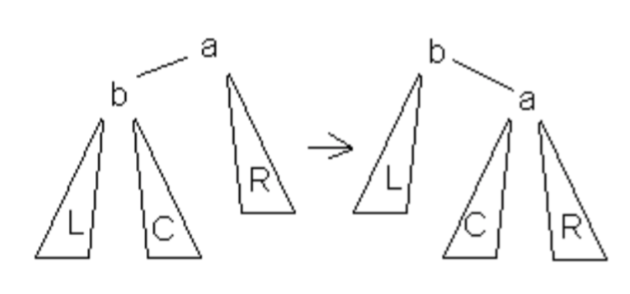
\includegraphics[width=7cm]{images/40-42_6.png}}
{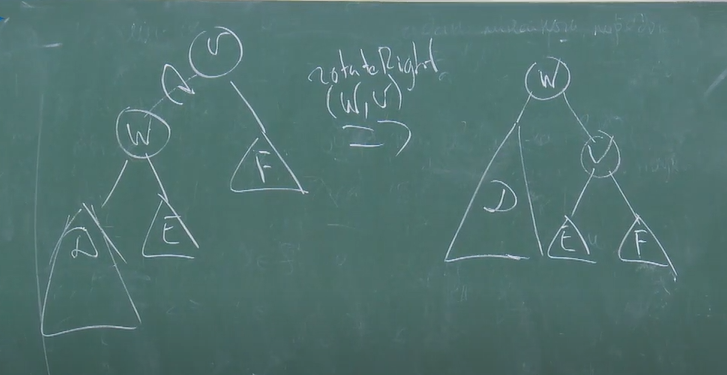
\includegraphics[width=7cm]{images/40-42_srr.PNG}}


\subsubsection*{Большой левый поворот}

\begin{itemize}
    \item Используется, когда $H(R) = H(L) + 1$ и $H(C) = H(L) + 2$
    \item После операции высота дерева уменьшается на 1
\end{itemize}

\begin{figure}[h]
\center{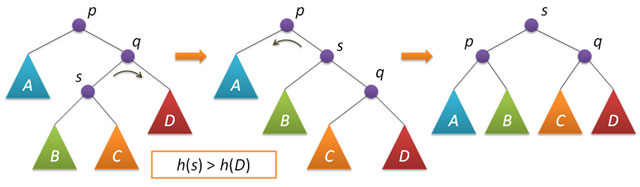
\includegraphics[width=10cm]{images/40-42_rotate.jpg}}
\end{figure}

\subsubsection*{Большой правый поворот}
\begin{figure}[h]
\center{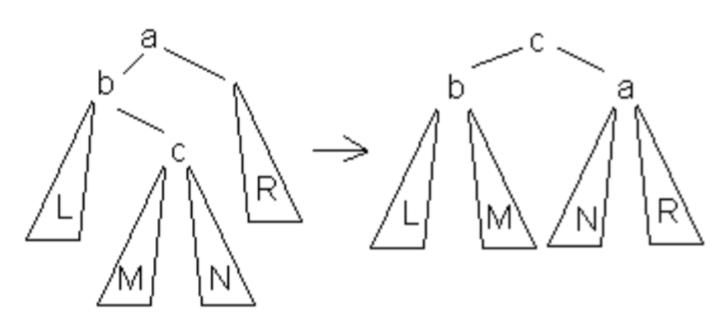
\includegraphics[width=7cm]{images/40-42_8.png}}
\end{figure}

\section{Большие и малые повороты в дереве поиска: сохранение свойств дерева}

\textbf{Корректность}

$\blacktriangle$ 
Рассмотрим итоговое дерево для малого поворота вправо:

Считаем, что до поворота дерево было корректным.

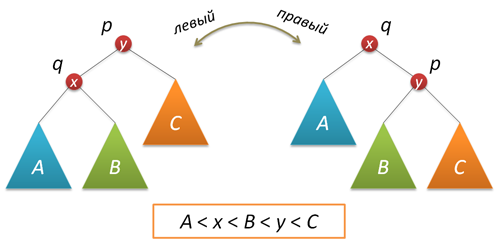
\includegraphics[width = 7cm]{images/40-42_smallrotate.png}

Так как все поддерево - это чей-то правый или левый ребенок, то не имеет значения, за какую вершину этого поддерева мы подвесим поддерево к родителю. Связь между родителем и q корректна.

A - левое поддерево q. До поворота оно тоже было левым поддеревом q, так что эта связь корректна.

q - левый ребенок p, поэтому p > q. Таким образом, связь между p и q в дереве после поворота корректна.

B  лежало в левом поддереве p, т.е. все значения B  меньше p. Значит, связь p-B корректна. B - правый ребенок q, поэтому то, что B лежит в правом поддереве q, тоже корректно.

С - правое поддерево p. До поворота оно тоже было правым поддеревом p, так что эта связь корректна. С лежало в правом поддереве p, а q - в левом. Поэтому C > q, так что то, что С лежит в правом поддереве q,  - корректно.

Для левого поворота аналогично.

Большой поворот - это комбинация 2х малых поворотов, поэтому большие повороты также корректны.

$\blacksquare$ 